\chapter{tracing the beam}
\lhead[tempest]{}
\label{sec:vector}
\lstset{style=6502Style}

\textit{Tempest} does its drawing to the screen using a piece of hardware called the 
\textit{Analog Vector Generator} (AVG). We can make this piece of kit draw stuff by supplying
it with operation codes (opcodes) that it treats as instructions for drawing lines to the
screen and updating their colour, position, and size. Most opcodes are a pair of bytes, since
this is usually enough to convey the necessary information. 
\begin{figure}[H]
  {
    \setlength{\tabcolsep}{3.0pt}
    \setlength\cmidrulewidth{\heavyrulewidth} % Make cmidrule = 
    \begin{adjustbox}{width=12.5cm,center}
      \begin{tabular}{lll}
        \toprule
        Description & OpCode Hex & Bitmap \\
        \midrule
        Draw relative vector.      & \icode{0x0\_\_\_ \_\_\_\_}   & \icode{000YYYYY YYYYYYYY IIIXXXXX XXXXXXXX} \\
                                   & \icode{0x1\_\_\_ \_\_\_\_}   & \icode{000YYYYY YYYYYYYY IIIXXXXX XXXXXXXX} \\
        Halt                       & \icode{0x2\_\_\_}        & \icode{00100000 00000000} \\
        Draw short relative vector & \icode{0x4\_\_\_}        & \icode{010YYYYY IIIXXXXX} \\
                                   & \icode{0x5\_\_\_}        & \icode{010YYYYY IIIXXXXX} \\
        New color/intensity        & \icode{0x6\_\_\_}        & \icode{0110URGB IIIIIIII} \\
        New scale                  & \icode{0x7\_\_\_}        & \icode{0111USSS SSSSSSSS} \\
        Center                     & \icode{0x8\_\_\_}        & \icode{10000000 00000000} \\
        Jump to subroutine         & \icode{0xA\_\_\_}        & \icode{101AAAAA AAAAAAAA} \\
                                   & \icode{0xB\_\_\_}        & \icode{101AAAAA AAAAAAAA} \\
        Return from subroutine     & \icode{0xC\_\_\_}        & \icode{11000000 00000000} \\
        Jump to new address        & \icode{0xE\_\_\_}        & \icode{111AAAAA AAAAAAAA} \\
                                   & \icode{0xF\_\_\_}        & \icode{111AAAAA AAAAAAAA} \\
      \end{tabular}
    \end{adjustbox}
  }
\end{figure}
\vspace{-0.5cm}
The table above lists all the 
known available opcodes for the AVG at the time that \textit{Tempest} was released. As you can
see, various values like the \icode{X} and \icode{Y} position, the color intensity (\icode{I}),
scale (\icode{S}), and memory address (\icode{A}) are encoded at the bit level in order to pack
them into the available byte pair. This means that there is a limit, for example, on the values
we can provide for things like \icode{X} and \icode{Y} positions: 4 bits in the 'Draw Short
Relative Vector' instruction allows values between 0 and 16 with an additional
fifth bit to indicate a positive or negative value.

So equipped with this table as our cheat sheet, let's imagine we want to start drawing something on the screen. First
we will move the beam to the centre of the screen:

\begin{figure}[H]
  {
    \setlength{\tabcolsep}{3.0pt}
    \setlength\cmidrulewidth{\heavyrulewidth} % Make cmidrule = 
    \begin{adjustbox}{width=6.5cm,center}
      \begin{tabular}{lll}
        \toprule
        Description & Op Code & Bitmap \\
        \midrule
        Center                     & \icode{0x8000}        & \icode{10000000 00000000} \\
      \end{tabular}
    \end{adjustbox}
  }
\end{figure}
So our opcode instruction is a two byte \icode{0x8000}. 
This thing we want to draw, we're going to make it yellow. So let's issue a colour command:

\begin{figure}[H]
  {
    \setlength{\tabcolsep}{3.0pt}
    \setlength\cmidrulewidth{\heavyrulewidth} % Make cmidrule = 
    \begin{adjustbox}{width=7.5cm,center}
      \begin{tabular}{lll}
        \toprule
        Description & Op Code & Bitmap \\
        \midrule
                                   & \icode{0x6\_\_\_}        & \icode{0110URGB IIIIIIII} \\
        Set Color to Yellow        & \icode{0x68C1}        & \icode{01101000 11000001} \\
      \end{tabular}
    \end{adjustbox}
  }
\end{figure}
In practice we find that our colour opcode always starts with \icode{0x68C}. In this instance we 
add a \icode{1} to set the color to yellow. To set it to red we would have used \icode{3} (i.e. \icode{0x68C3}).
To set it to blue we would have used \icode{7} (i.e. \icode{0x68C7}). The values are abitrary, but you get the idea.

Now we're ready to draw. Let's project a line 4 units to the right and 2 units down:

\begin{minipage}[c]{0.68\linewidth}
\begin{figure}[H]
  {
    \catcode32=\active
    \setlength{\tabcolsep}{3.0pt}
    \setlength\cmidrulewidth{\heavyrulewidth} % Make cmidrule = 
    \begin{adjustbox}{width=7.5cm,center}
      \begin{tabular}{lll}
        \toprule
        Description & Op Code & Bitmap \\
        \midrule
                                   & \icode{0x5\_\_\_}        & \icode{010YYYYY IIIXXXXX} \\
          Draw vector to (4,-2)    & \icode{0x5EC4}          & \icode{01011110 11000100} \\
                                   &                         & \icode{   5   E    C   4} \\
      \end{tabular}
    \end{adjustbox}
  }
\end{figure}
\end{minipage}
\hspace{0.1cm}
\begin{minipage}[c]{0.30\linewidth}
\begin{figure}[H]
    \centering
    \begin{adjustbox}{width=4.5cm,center}
      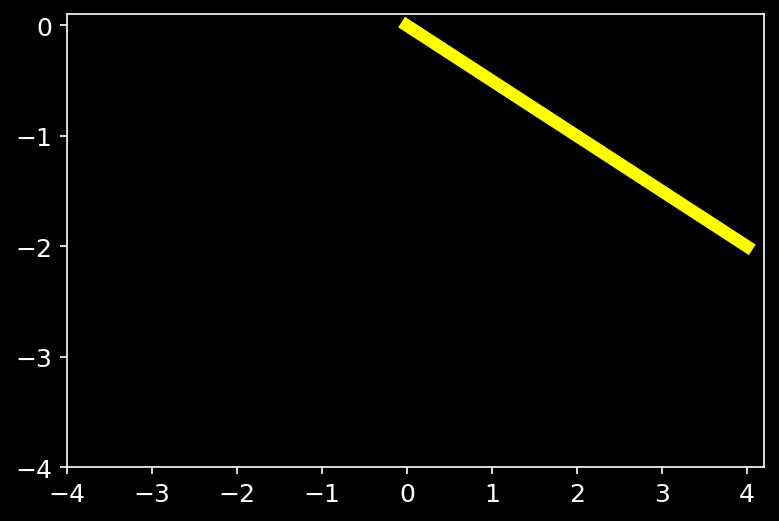
\includegraphics[width=12cm]{src/lifes/build_cursor_3_6.png}%
    \end{adjustbox}
\end{figure}
\end{minipage}

Now you might notice something that gives you pause. Where we have added the \icode{4}
in our vector opcode is relatively obvious (at the end of \icode{5EC4}). But why has
the -2 become an \icode{E}? Shouldn't it be \icode{52C4} instead?

The answer is \textit{two's complement}. This is the way we represent negative numbers. The first
bit under the first \icode{Y} above tells us that what we have is a negative number (it's why the opcode
begins with a \icode{4} instead of a \icode{5}). But for the remaining 4 bits of our \icode{Y}
value the following mapping applies:

\begin{minipage}[c]{0.48\linewidth}
  \begin{figure}[H]
    {
      \catcode32=\active
      \setlength{\tabcolsep}{3.0pt}
      \setlength\cmidrulewidth{\heavyrulewidth} % Make cmidrule = 
      \begin{adjustbox}{width=4.5cm,center}
        \begin{tabular}{llll}
          \toprule
          Decimal & Hexadecimal \\
          \midrule
          -1 & \icode{F} \\
          -2 & \icode{E} \\
          -3 & \icode{D} \\
          -4 & \icode{C} \\
          -5 & \icode{B} \\
          -6 & \icode{A} \\
          -7 & \icode{9} \\
          -8 & \icode{8} \\
          -9 & \icode{7} \\
        \end{tabular}
      \end{adjustbox}
    }\caption*{Negative Values}
  \end{figure}
\end{minipage}
\hspace{0.1cm}
\begin{minipage}[c]{0.48\linewidth}
  \begin{figure}[H]
    {
      \catcode32=\active
      \setlength{\tabcolsep}{3.0pt}
      \setlength\cmidrulewidth{\heavyrulewidth} % Make cmidrule = 
      \begin{adjustbox}{width=4.5cm,center}
        \begin{tabular}{llll}
          \toprule
          Decimal & Hexadecimal \\
          \midrule
           1 & \icode{1}\\
           2 & \icode{2}\\
           3 & \icode{3}\\
           4 & \icode{4}\\
           5 & \icode{5}\\
           6 & \icode{6}\\
           7 & \icode{7}\\
           8 & \icode{8}\\
           9 & \icode{9}\\
        \end{tabular}
      \end{adjustbox}
    }\caption*{Positive Values}
  \end{figure}
\end{minipage}


As you can see, to represent negative integers with \textit{two's complement}, we 'start again' at
\icode{F} and count downwards. So to represent a value of -2 we use \icode{E}.

With this in mind we can start drawing again. This time we want to move left 3 units and down 1
unit. So we issue the opcode command \icode{0x5FDD} to the vector generator:

\begin{minipage}[c]{0.68\linewidth}
\begin{figure}[H]
  {
    \catcode32=\active
    \setlength{\tabcolsep}{3.0pt}
    \setlength\cmidrulewidth{\heavyrulewidth} % Make cmidrule = 
    \begin{adjustbox}{width=7.5cm,center}
      \begin{tabular}{lll}
        \toprule
        Description & Op Code & Bitmap \\
        \midrule
                                   & \icode{0x5\_\_\_}        & \icode{010YYYYY IIIXXXXX} \\
          Draw vector to (-3,-1)    & \icode{0x5FDD}          & \icode{01011111 11011101} \\
                                   &                          & \icode{   5   F    D   D} \\
      \end{tabular}
    \end{adjustbox}
  }
\end{figure}
\end{minipage}
\hspace{0.1cm}
\begin{minipage}[c]{0.30\linewidth}
\begin{figure}[H]
    \centering
    \begin{adjustbox}{width=4.5cm,center}
      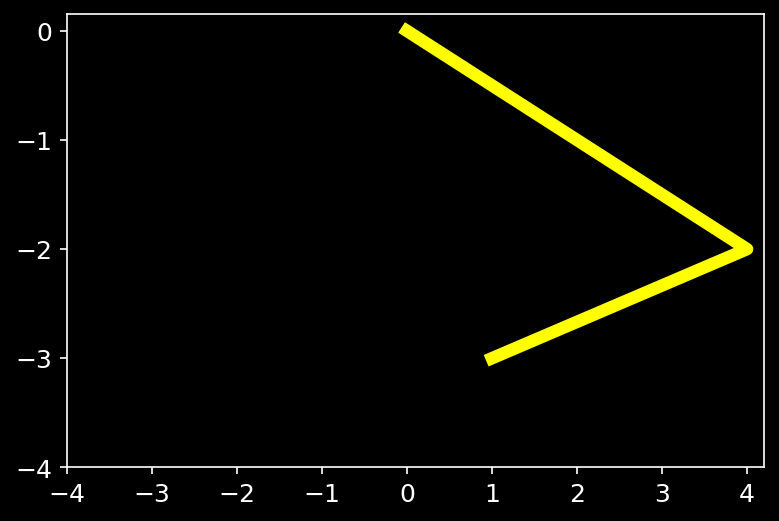
\includegraphics[width=12cm]{src/lifes/build_cursor_4_6.png}%
    \end{adjustbox}
\end{figure}
\end{minipage}

Next we move right 2 units and up 1 unit:

\begin{minipage}[c]{0.68\linewidth}
\begin{figure}[H]
  {
    \catcode32=\active
    \setlength{\tabcolsep}{3.0pt}
    \setlength\cmidrulewidth{\heavyrulewidth} % Make cmidrule = 
    \begin{adjustbox}{width=7.5cm,center}
      \begin{tabular}{lll}
        \toprule
        Description & Op Code & Bitmap \\
        \midrule
                                   & \icode{0x4\_\_\_}        & \icode{0100YYYY IIIXXXXX} \\
            Draw vector to (2,1)   & \icode{0x41C2}          & \icode{01000001 11000010} \\
                                   &                          & \icode{   4   1    C   2} \\
      \end{tabular}
    \end{adjustbox}
  }
\end{figure}
\end{minipage}
\hspace{0.1cm}
\begin{minipage}[c]{0.30\linewidth}
\begin{figure}[H]
    \centering
    \begin{adjustbox}{width=4.5cm,center}
      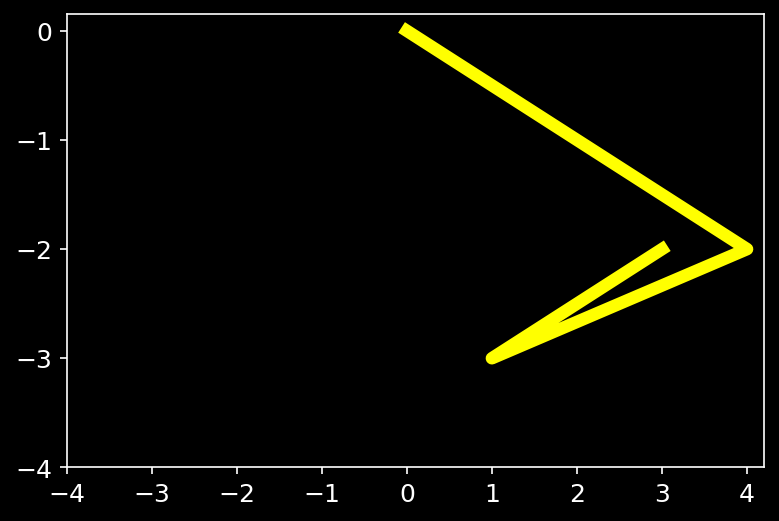
\includegraphics[width=12cm]{src/lifes/build_cursor_5_6.png}%
    \end{adjustbox}
\end{figure}
\end{minipage}

Then left 3 units and up 1 unit:

\begin{minipage}[c]{0.68\linewidth}
\begin{figure}[H]
  {
    \catcode32=\active
    \setlength{\tabcolsep}{3.0pt}
    \setlength\cmidrulewidth{\heavyrulewidth} % Make cmidrule = 
    \begin{adjustbox}{width=7.5cm,center}
      \begin{tabular}{lll}
        \toprule
        Description & Op Code & Bitmap \\
        \midrule
                                   & \icode{0x4\_\_\_}        & \icode{0100YYYY IIIXXXXX} \\
          Draw vector to (-3,1)    & \icode{0x41DD}          & \icode{01000001 11011101} \\
                                   &                          & \icode{   4   1    D   D} \\
      \end{tabular}
    \end{adjustbox}
  }
\end{figure}
\end{minipage}
\hspace{0.1cm}
\begin{minipage}[c]{0.30\linewidth}
\begin{figure}[H]
    \centering
    \begin{adjustbox}{width=4.5cm,center}
      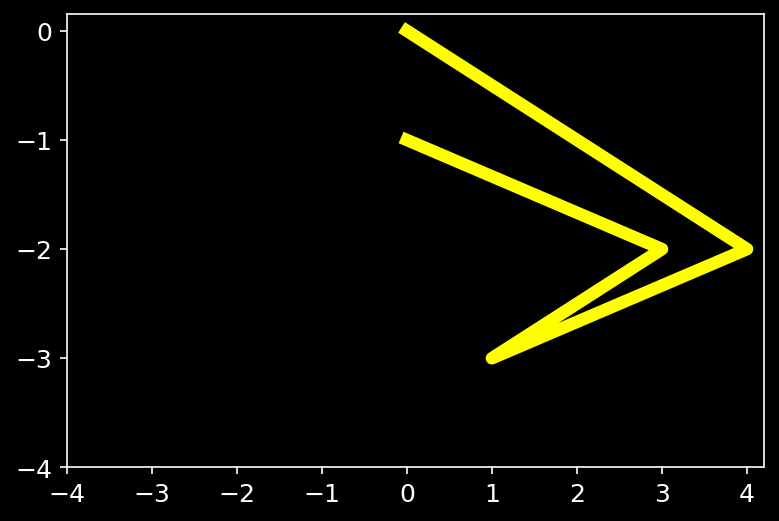
\includegraphics[width=12cm]{src/lifes/build_cursor_6_6.png}%
    \end{adjustbox}
\end{figure}
\end{minipage}

Things are starting to take shape. Can you guess what we're drawing yet? Our next line will
go left 3 units and down 1 unit:

\begin{minipage}[c]{0.68\linewidth}
\begin{figure}[H]
  {
    \catcode32=\active
    \setlength{\tabcolsep}{3.0pt}
    \setlength\cmidrulewidth{\heavyrulewidth} % Make cmidrule = 
    \begin{adjustbox}{width=7.5cm,center}
      \begin{tabular}{lll}
        \toprule
        Description & Op Code & Bitmap \\
        \midrule
                                   & \icode{0x5\_\_\_}        & \icode{010YYYYY IIIXXXXX} \\
        Draw vector to (-3,-1)    & \icode{0x5FDD}          & \icode{01011111 11011101} \\
                                   &                          & \icode{   5   F    D   D} \\
      \end{tabular}
    \end{adjustbox}
  }
\end{figure}
\end{minipage}
\hspace{0.1cm}
\begin{minipage}[c]{0.30\linewidth}
\begin{figure}[H]
    \centering
    \begin{adjustbox}{width=4.5cm,center}
      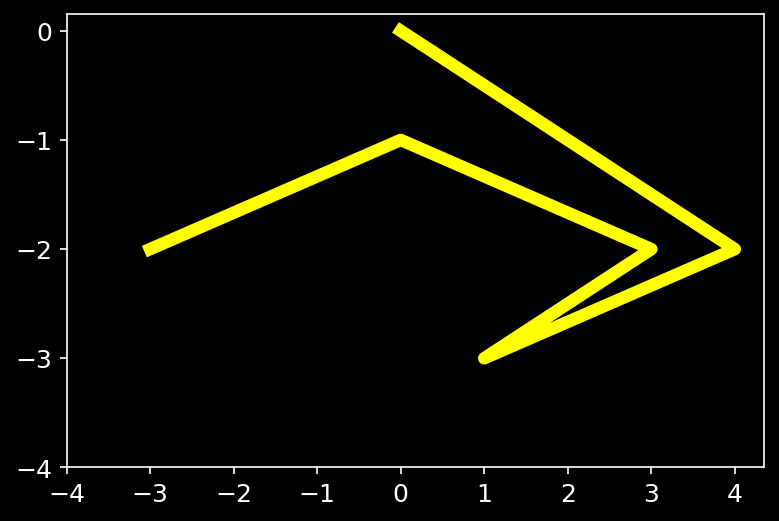
\includegraphics[width=12cm]{src/lifes/build_cursor_7_6.png}%
    \end{adjustbox}
\end{figure}
\end{minipage}

OK I think you can see how we're building up our picture here, so let's get it over with:

\begin{minipage}[c]{0.68\linewidth}
\begin{figure}[H]
  {
    \catcode32=\active
    \setlength{\tabcolsep}{3.0pt}
    \setlength\cmidrulewidth{\heavyrulewidth} % Make cmidrule = 
    \begin{adjustbox}{width=7.5cm,center}
      \begin{tabular}{lll}
        \toprule
        Description & Op Code & Bitmap \\
        \midrule
                                   & \icode{0x5\_\_\_}        & \icode{010YYYYY IIIXXXXX} \\
          Draw vector to (2,-1)    & \icode{0x5FC2}          & \icode{01011111 11000010} \\
                                   &                          & \icode{   5   F    C   2} \\
      \end{tabular}
    \end{adjustbox}
  }
\end{figure}
\end{minipage}
\hspace{0.1cm}
\begin{minipage}[c]{0.30\linewidth}
\begin{figure}[H]
    \centering
    \begin{adjustbox}{width=4.5cm,center}
      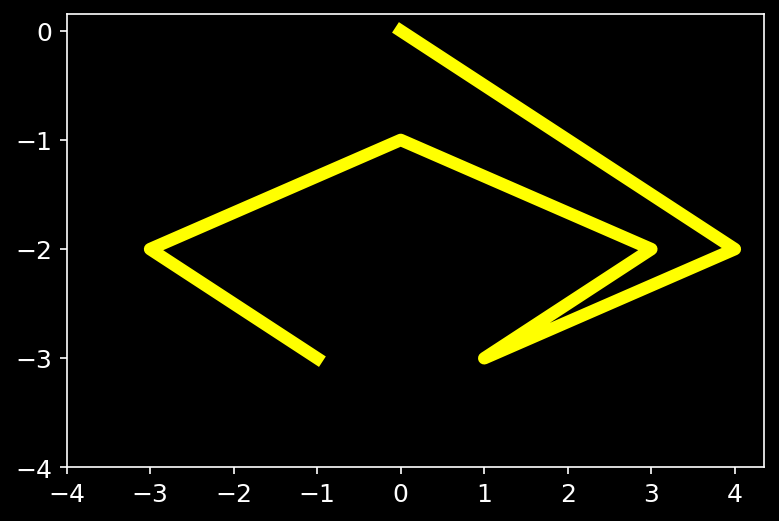
\includegraphics[width=12cm]{src/lifes/build_cursor_8_6.png}%
    \end{adjustbox}
\end{figure}
\end{minipage}


\begin{minipage}[c]{0.68\linewidth}
\begin{figure}[H]
  {
    \catcode32=\active
    \setlength{\tabcolsep}{3.0pt}
    \setlength\cmidrulewidth{\heavyrulewidth} % Make cmidrule = 
    \begin{adjustbox}{width=7.5cm,center}
      \begin{tabular}{lll}
        \toprule
        Description & Op Code & Bitmap \\
        \midrule
                                   & \icode{0x4\_\_\_}        & \icode{0100YYYY IIIXXXXX} \\
          Draw vector to (-3,1)    & \icode{0x41DD}          & \icode{01000001 11011101} \\
                                   &                          & \icode{   4   1    D   D} \\
      \end{tabular}
    \end{adjustbox}
  }
\end{figure}
\end{minipage}
\hspace{0.1cm}
\begin{minipage}[c]{0.30\linewidth}
\begin{figure}[H]
    \centering
    \begin{adjustbox}{width=4.5cm,center}
      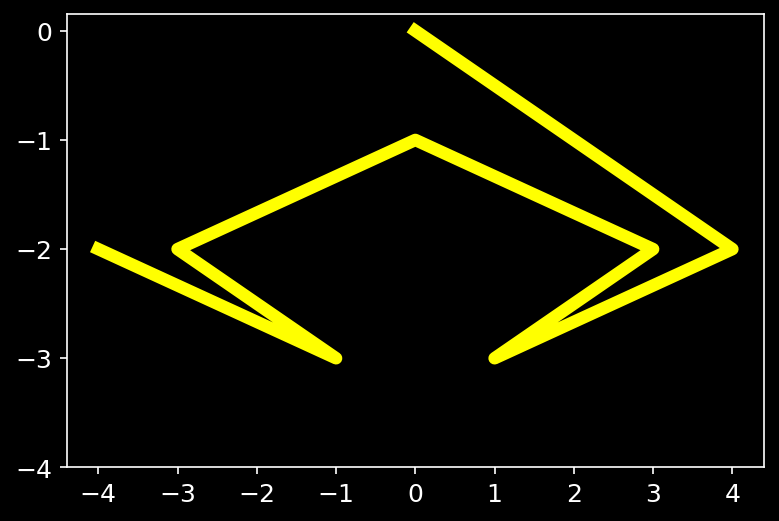
\includegraphics[width=12cm]{src/lifes/build_cursor_9_6.png}%
    \end{adjustbox}
\end{figure}
\end{minipage}

\begin{minipage}[c]{0.68\linewidth}
\begin{figure}[H]
  {
    \catcode32=\active
    \setlength{\tabcolsep}{3.0pt}
    \setlength\cmidrulewidth{\heavyrulewidth} % Make cmidrule = 
    \begin{adjustbox}{width=7.5cm,center}
      \begin{tabular}{lll}
        \toprule
        Description & Op Code & Bitmap \\
        \midrule
                                   & \icode{0x4\_\_\_}        & \icode{0100YYYY IIIXXXXX} \\
            Draw vector to (4,2)    & \icode{0x42C4}          & \icode{01000010 11000100} \\
                                   &                          & \icode{   4   2    C   4} \\
      \end{tabular}
    \end{adjustbox}
  }
\end{figure}
\end{minipage}
\hspace{0.1cm}
\begin{minipage}[c]{0.30\linewidth}
\begin{figure}[H]
    \centering
    \begin{adjustbox}{width=4.5cm,center}
      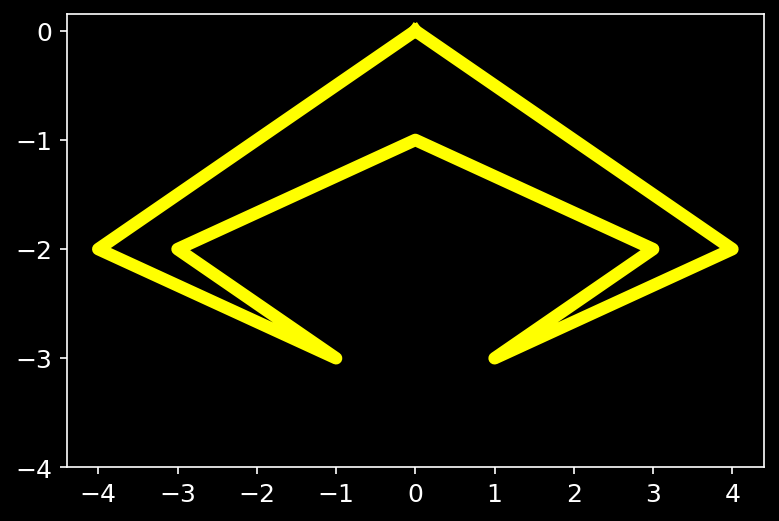
\includegraphics[width=12cm]{src/lifes/build_cursor_10_6.png}%
    \end{adjustbox}
\end{figure}
\end{minipage}

And there it is. We've drawn the 'lives left' symbol used in \textit{Tempest} to indicate the number
of player lives remaining. Not bad for a handful of bytes.

Before signing off, let's look at the dense little assembler macro used to construct these opcode
values. This function, called \icode{VCTR}, takes a pair of X and Y values, e.g. (4,2), as well as a color intensity value,
and converts them into the packed two-byte opcode. It is an object lesson in old-school bit
manipulation written by Ed Logg in 1979 to support the original version of the Analogue Vector
Generator. As we read more about \textit{Tempest} we'll find that Dave Theurer's source code
makes heavy use of it when drawing player and enemy to the screen.

\begin{lstlisting}
;
;       VCTR - DRAW VECTOR INSTRUCTION
;       THIS INSTRUCTION DRAWS A VECTOR ON THE DISPLAY AREA
;       RELATIVE TO THE PREVIOUS BEAM POSITION BEFORE THE
;       INSTRUCTION IS EXECUTED.  DX IS THE CHANGE IN BEAM X
;       POSITION; DY IS THE CHANGE IN BEAM Y POSITION; ZZ 
;       SPECIFIES THE BEAM INTENSITY (0 THROUGH 7., 0 IS
;       NO INTENSITY, 7. IS BRIGHTEST INTENSITY).
;
        .SBTTL  VCTR
        .MACRO  VCTR DX,DY,ZZ
        ...1=DX                    ; STORE X ARG IN ...1
        ...2=DY                    ; STORE Y ARG IN ...2
        .IF      LT,...1           ; IF NEGATIVE X
        ...1=-DX                   ; CONVERT TO TWO'S COMPLEMENT.
        .ENDC                      ; END IF
        .IF      LT,...2           ; IF NEGATIVE Y
        ...2=-DY                   ; CONVERT TO TWO'S COMPLEMENT.
        .ENDC                      ; END IF
        ...5=...1!...2             ; OR X AND Y TOGETHER IN ...5
    
        .IF     NE,...1+...2       ; IF X AND Y ARE 0 - SKIP SHORT VECTOR
        .IF      EQ,...5&^H0FFE1   ; IF WE HAVE AN X OR Y VALUE..
        ; DRAW IT WITH A SHORT VECTOR OPCODE.
        ; THE BITMAP FOR THIS IS: 010YYYYY IIIXXXXX
        ; BRIEF EXPLANATION OF THE BIT MANIPULATIONS:
        ; ^H4000 - HEX 4000 IS OUR BASE FOR SHORT VECTOR OPCODE.
        ; <ZZ*^H20> - MOVE THE INTENSITY VALUE TO THE III SLOT ABOVE.
        ; <DX/2&^H1F> - MOVE THE X VALUE TO THE END OF THE 2ND BYTE.
        ; <DY*^H80&^H1F00> - MOVE THE Y VALUE TO THE END OF THE 1ST BYTE.
        .WORD   ^H4000+<ZZ*^H20>+<DX/2&^H1F>+<DY*^H80&^H1F00>
        .MEXIT                     ; EXIT MACRO.
        .ENDC                      ; END IF
        .ENDC                      ; OTHERWISE..
        ; DRAW AS A RELATIVE VECTOR, WHICH ALLOWS FOR LARGER VALUES.
        ; THE BITMAP FOR THIS IS 4 BYTES LONG:
        ;   000YYYYY YYYYYYYY IIIXXXXX XXXXXXXX
        ; DY&^H1FFF - PUT THE Y VALUE IN 2ND BYTE OF 1ST BYTE PAIR.
        ; <ZZ*^H2000> INTENSITY VALUE AT START OF 1ST BYTE IN 2ND PAIR.
        ; <DX&^H1FFF> X VALUE IN 2ND BYTE OF 2ND BYTE PAIR.
        .WORD   DY&^H1FFF,<ZZ*^H2000>+<DX&^H1FFF>
        .ENDM                      ; END MACRO
\end{lstlisting}
